\documentclass[tikz,border=3.14mm]{standalone}
\usepackage{tikz}


\begin{document}
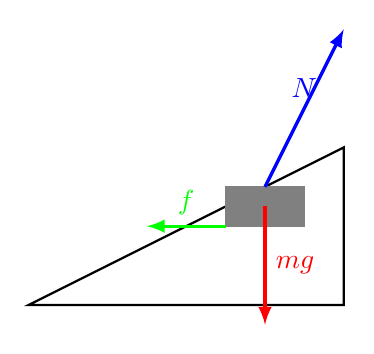
\begin{tikzpicture}[>=latex]

% Draw the inclined plane
\draw[thick] (0,0) -- (4,0) -- (4,2) -- cycle;

% Draw the block
\filldraw [gray] (2.5,1) rectangle (3.5,1.5);

% Draw and label the weight force
\draw[->, very thick, red] (3,1.25) --+ (0,-1.5) node[midway,right] {$mg$};

% Draw and label the normal force
\draw[->, very thick, blue] (3,1.5) --+ (1,2) node[midway,above] {$N$};

% Draw and label the friction force
\draw[->, very thick, green] (2.5,1) --+ (-1,0) node[midway,above] {$f$};

\end{tikzpicture}
\end{document}